\chapter{Realisierung}\label{chapter:realization}
%%%%%%%%%%%%%%%%%%%%%%%%%%%%%%%%%%%%%%%%%%%%%%%%%%%%%%%%%%%%
%\imiscomment{Beschreibung der hard- und software-technischen Realisierung}
%
%\imiscomment{Struktur dieses Kapitel kann je nach Problemstellung unterschiedlich gestaltet werden}
%%%%%%%%%%%%%%%%%%%%%%%%%%%%%%%%%%%%%%%%%%%%%%%%%%%%%%%%%%%%
\section{Realisierung der Einzelmodule}
%%%%%%%%%%%%%%%%%%%%%%%%%%%%%%%%%%%%%%%%%%%%%%%%%%%%%%%%%%%%

%%%%%%%%%%%%%%%%%%%%%%%%%%%%%%%%%%%%%%%%%%%%%%%%%%%%%%%%%%%%
\subsection{SimulationEngine und SimulationClock}\label{subsec:real_engine}
\subsubsection{SimulationEngine}
Die \codeclass{SimulationEngine} ist als Singleton realisiert. Dies hat den Vorteil, dass es zur Laufzeit nur eine Instanz von ihr geben kann, die in allen Klassen verfügbar ist. Diese Instanz hält die \codeclass{World}, den \codeclass{CommunicationHandler} bereit. Beide Objekte können vor dem Start der Simulation, d.h. vor dem Start der \codeclass{SimulationClock} mit den jeweiligen Setter-Methoden gesetzt werden. Der Aufruf dieser Methoden nach dem Start der Simulation erzeugt einen \codeclass{IllegalAccessException}.

Während der Simulation können die Welt und der Kommunikationshandler über die Getter-Methoden abgerufen werden. Auf diesem Weg können unter anderem Sensoren und Aktuatoren den Kommunikationshandler erreichen. Auch die graphische Oberfläche holt sich die zu zeichnenden Objekte über die Simulationsengine.

\subsubsection{SimulationClock}
Die \codeclass{SimulationClock} ist das Herzstück der Simulation. Sie stößt sämtliche Aktionen der Komponenten des Modells an. Die Clock ist wie die Engine ebenfalls mit dem Singleton-Designpatter realisiert. So ist sicher gestellt, dass es nur eine Uhr geben kann, die aus allen Klassen erreichbar ist.

Die \codeclass{SimulationClock} verwendet das Listener-Konzept, um Komponenten, die an der Simulationszeit interessiert sind regelmäßig über Änderungen zu informieren. Komponenten die sich als Listener bei der Uhr registrieren möchten müssen dazu die \codeinterface{ISimulationClockListener}-Schnittstelle implementieren und können dann mit 
\begin{illfloat}[H]
  \begin{lstlisting}
SimulationClock.getInstance()
.addListener(ISimulationClockListener);
  \end{lstlisting}
  \illcaption{Beispiel für das Hinzufügen eines Listeners an die SimulationClock}
\end{illfloat}

hinzugefügt und analog mit
\begin{illfloat}[H]
\begin{lstlisting}
SimulationClock.getInstance()
.removeListener(ISimulationClockListener);
\end{lstlisting}
  \illcaption{Beispiel für das Entfernen eines Listeners an die SimulationClock}
\end{illfloat}
wieder entfernt werden.

Über das Listener-Konzept werden in jeder simulierten Sekunde Aktionen bei den Listenern angestoßen. Standardmäßig ist es nicht möglich, eine Java-Collection während des Durchlaufens dieser zu verändern. Somit wäre es unmöglich, dass sich eine Komponente als Listener abmelden kann. Die \codeclass{SimulationClock} speichert jedoch alle Hinzufüge- und Entfernanfragen an die Listener-Collection zwischen und führt diese vor dem nächsten Durchlauf aus.

Die Uhr basiert auf einem Timer-Thread, der alle $x$ Millisekunden auslöst. Wenn die Uhrzeit skaliert wird, wird mit dem nächsten Tick ein neuer Timer eingerichtet. Das Pausieren der Simulation stoppt nicht den Timer-Thread sondern verhindert lediglich, dass dieser die \codeclass{SimulationTime} inkrementiert.
%%%%%%%%%%%%%%%%%%%%%%%%%%%%%%%%%%%%%%%%%%%%%%%%%%%%%%%%%%%%


%%%%%%%%%%%%%%%%%%%%%%%%%%%%%%%%%%%%%%%%%%%%%%%%%%%%%%%%%%%%
\subsection{Generatoren}\label{subsec:real_generator}
%%%%%%%%%%%%%%%%%%%%%%%%%%%%%%%%%%%%%%%%%%%%%%%%%%%%%%%%%%%%
Für das Erstellen einer neuen Simulation reicht es aus, eine Simulationswelt (der Klasse \codeclass{World}) zu erzeugen. Dieser Vorgang wird als Generierung bezeichnet und von einem Generator realisiert.
Ein Beispiel, wie eine solche erzeugt werden kann, ist in diesem Kapitel an Hand der Demonstrationssimulation dargestellt.\\ 

Aus Modularitätsgründen haben wir uns für das Konzept eines leicht austauschbaren Generators entschieden. Dafür wurde die Schnittstelle \codeinterface{IWorldGenerator} entworfen, welches nur eine Methode (\codemethod{generateWorld()}) definiert, die von allen konkreten Generatoren als Schnittstelle genutzt werden sollte.
Darüber hinaus gibt es im Generatorpaket (\codeinline{de.uniluebeck.imis.casi.gene\-rator}) einige Helferklassen, deren Name mit \codeclass{Collector} gekennzeichnet ist und einen \codeclass{Linker}.\\

Durch den gewählten Ansatz der starken Abstraktion ist es möglich Simulationen auf die unterschiedlichsten Arten zu beschreiben ohne Änderungen am Simulator vornehmen zu müssen. Das von uns gewählte, am kurzfristigsten umzusetzende Vorgehen ist es, direkt aus Java-Klassen heraus die Objekte der Simulationswelt zu erzeugen und zu verknüpfen. Weitere Möglichkeiten wären:
\begin{itemize}
  \item{Beschreibungssprachen wie XML, YML oder JSon}
  \item{Erzeugung durch eine eingebettete Skriptsprache wie LUA oder JRuby}
\end{itemize}
In einem frühen Konzept unserer Projektarbeit war insbesondere eine Beschreibung durch eine spezifizierte XML (Arbeitstitel: \codeinline{CASiX}) vorgesehen. Diese wurde jedoch im Laufe des Semesters wegen nicht unerheblichen Aufwand zurückgestellt. Da eine saubere und klare Schnittstelle definiert wurde, ist es ohne Weiteres möglich, dass diese später noch hinzugefügt werden.

\subsubsection{Generierung durch Java-Code}\label{subsec:real_generator_java}
Für das Erstellen einer neuen Simulation hat es sich als sinnvoll erwiesen, ein neues Paket zu erstellen und darin die \codeinterface{IWorld\-Generator}-Schnittstelle zu implementieren. Innerhalb dieses Paketes ist eine Aufteilung in weitere Klasse zu empfehlen.

\begin{figure}[htb]
  \begin{center}
    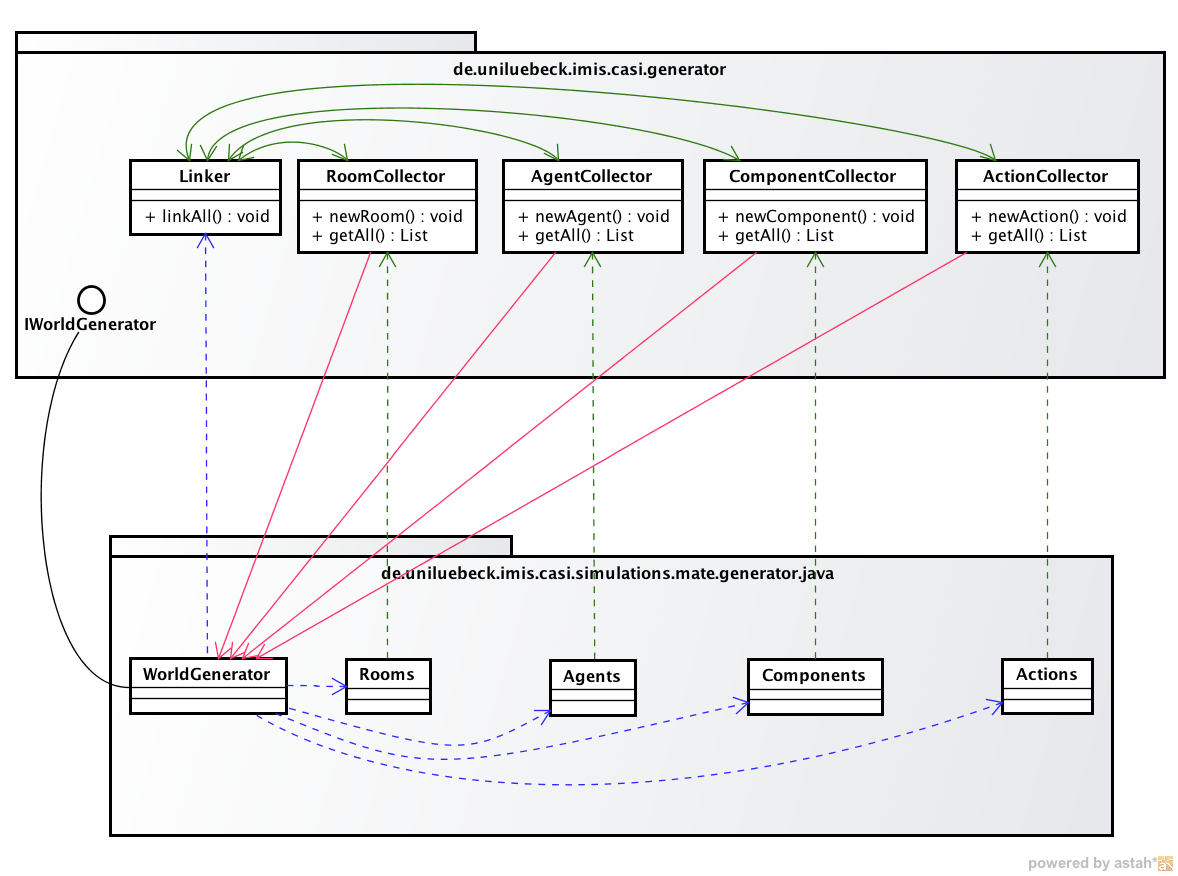
\includegraphics[width=\textwidth]{pics/howToGenerateAWorld.png}
  \end{center}
  \caption{abgewandeltes UML-Klassendiagramm zur Darstellung der Aufteilung eines Generators. Blau gestrichelt: Aufruf statischer Methoden, grün gestrichelt: einfügen von Objekten, grün: Verknüpfung von Objekten untereinander, rot: entgegennehmen von gesammelten Objekten}
  \label{fig:howToGenerateAWorld}
\end{figure}
In Abbildung \ref{fig:howToGenerateAWorld} ist, exemplarisch an unserer Demosimulation, eine solche Aufteilung gezeigt.
Dort ist das untere Paket für die MATe-Simulation zu sehen. Darin: der eigentliche \codeclass{World\-Generator}, welcher die zu generierenden Teile durch Aufrufe von statischen Methoden an die andere Klassen delegiert. Hier gezeigt durch gestrichelten blauen Linien.
Die jeweiligen Klassen (alle als \codeinline{static} deklariert), arbeiten dann die, in ihnen beschriebenen, Java-Ausdrücke ab.
Daraus resultierende Objekte werden in den, vom CASi-Kern bereitgestellten, Kollektoren gesammelt (gestrichelte grüne Pfeile). Die Reihenfolge der Erzeugung ist besonders zu beachten, da für einige Objekte andere bereits vorhanden sein müssen. Es hat sich die Reihenfolge: erst Räume, dann Agenten, dann Sensoren und Aktuatoren und schlussendlich Aktionen etabliert.
Wenn alle Erzeugerklassen abgearbeitet sind, ruft der \codeclass{World\-Generator} den \codeclass{Linker} auf. Dieser ist auch vom CASi-Kern bereitgestellt. Er übernimmt das Verknüpfen der Objekte untereinander, so zum Beispiel das Hinzufügen der für die Agenten erzeugten Aktionen in deren Todo-Liste.
Als letzten Schritt nimmt der Generator alle Komponenten (rote Pfeile) und erzeugt daraus ein \codeclass{World}-Objekt.

%%%%%%%%%%%%%%%%%%%%%%%%%%%%%%%%%%%%%%%%%%%%%%%%%%%%%%%%%%%%
\subsection{Benutzungsschnittstellen}\label{subsec:real_interfaces}
%%%%%%%%%%%%%%%%%%%%%%%%%%%%%%%%%%%%%%%%%%%%%%%%%%%%%%%%%%%%

Als Benutzungsschnittstelle für den Simulator haben wir die \emph{Simple GUI} entwickelt. Diese soll die simulierte Welt grafisch darstellen und es ermöglichen, gewünschte Informationen abzurufen. Wir wollten, dass diese Benutzungsschnittstelle sowohl für die späteren Hauptbenutzer, die Simulationen testen, viele Funktionen bietet, aber auch für Benutzer verständlich ist, die von dem System noch keine fortgeschrittenen Kenntnisse haben. Zum Beispiel könnte sie auch benutzt werden, um anderen das MACK-Framework zu präsentieren und zu veranschaulichen.

Die \emph{Simple GUI} ist eines der Module des Simulators, die sich leicht durch ein passendes anderes ersetzen lassen. Wenn also beispielsweise die angezeigten Informationen nicht ausreichend oder für bestimmte Simulationen überflüssig und deshalb störend sind, kann man die Benutzungsschnittstelle austauschen. Realisiert wird dies durch das Interface \codeinterface{IMainView}, die neue Schnittstelle muss bei der Implementierung dieses Interface benutzen. Ein ganz einfaches Beispiel für eine Implementierung ist die Klasse \codeclass{GuiStub}, die eingesetzt wird, wenn keine grafische Benutzungsschnittstelle erwünscht ist.

Für die graphische Oberfläche benutzen wir die Swing-Bibliothek, da wir aus dem Praktikum \emph{Softwaretechnik} einige Erfahrung mit der Swing-Entwicklung haben.

Die \emph{Simple GUI} ist aufgebaut, wie in Abbildung \ref{fig:simplegui-screen} zu sehen ist. Im Simulationsbereich (rot) wird die simulierte Welt gezeichnet. Der Informationsbereich (grün) an der rechten Seite bietet dem Benutzer die Möglichkeit detaillierte Informationen über Simulationskomponenten abzufragen. Zwischen dem Simulationsbereich und dem Informationsbereich befindet sich ein verschiebbare Trennung. Der Steuerungsbereich (blau) im unteren Teil lässt den Benutzer eingeschränkt Einfluss auf die Simulation nehmen. Die Menüleiste (gelb) im oberen Bildbereich bietet einige grundlegende Programmfunktionen. Letztere sollte in einem im Fenster ausgeführten Programm nicht fehlen, da sie den meisten Benutzern vertraut ist und ihr Fehlen für eine gewisse Hilflosigkeit sorgen könnte. 

\begin{figure}[htb]
  \begin{center}
    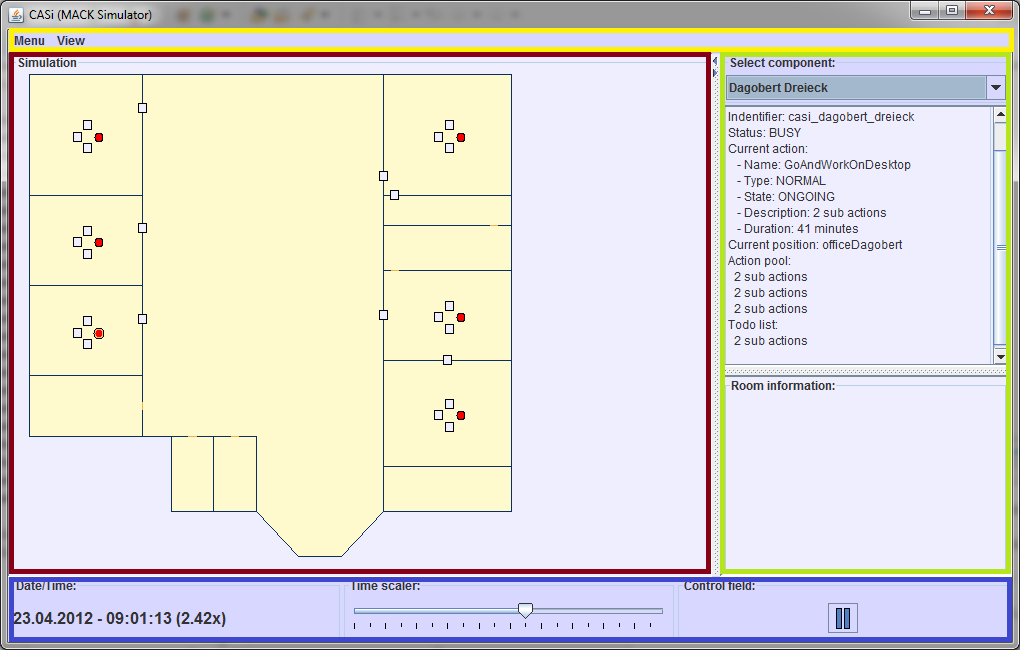
\includegraphics[width=\textwidth]{pics/screen2.png}
  \end{center}
  \caption{Screenshot der Anwendung}
  \label{fig:simplegui-screen}
\end{figure}

Der Simulationsbereich besteht aus einer \codeclass{JLayeredPane}. Auf dieser wiederum gibt es drei Ebenen:

\begin{itemize}
\item Ebene 1: Auf der tiefsten Ebene wird der Hintergrund gezeichnet. Dazu gehören die Räume mit ihren Wänden und Türen und die Einflussbereiche der Sensoren. Außerdem werden einige weitere, für das Debugging wichtige Elemente dargestellt, wie die zentralen Punkte der Räume und der Türen. Ebenfalls auf dieser Ebene liegen die Labels für Sensoren, Räume und Türen. In ungünstigen Fällen können sich die Bezeichner im Simulationsbereich überschneiden. Da aber die Identifizierung der Komponenten trotzdem möglich ist und die Berechnung für Bezeichnerposition und -größe für beliebige Simulationen recht schwierig ist, haben wir uns entschieden, das Problem zu vernachlässigen.

\item Ebene 2: Auf dieser Ebene liegen die Sensoren und Aktuatoren. Diese sind ein wesentlicher Bestandteil der Simulation und sollen deshalb nicht durch Teile des Hintergrundes verdeckt werden. Jedes dieser Komponenten wird dargestellt mit Hilfe der Klasse \codeclass{InteractionCom\-ponentView}, die von \codeclass{ComponentView} erbt, welche wiederum eine \codeclass{JComponent} ist. Ein Sensor oder Aktuator wird gezeichnet als ein Quadrat mit der Hintergrundfarbe der Simulation. Da die Sensoren und Aktuatoren beliebig viele Zustände annehmen können, haben wir darauf verzichtet zu implementieren, dass ihr Zustand an der Färbung erkennbar ist.

\item Ebene 3: Auf der obersten Ebene befinden sich die Agenten. Diese haben wir als wichtigsten Bestandteil der Simulation eingestuft, deshalb sollen sie durch nichts anderes überdeckt werden. Jeder Agent wird dargestellt mittels der von uns implementierten Klasse \codeclass{AgentView}, die ebenfalls von \codeclass{ComponentView} erbt. Die Klasse \codeclass{AgentView} implementiert das Interface \codeinterface{IAgentListener}. Mit den Methoden \codemethod{state\-Changed(STATE new\-State,\- Agent agent)} und \codemethod{position\-Changed(Point2D oldPosition, Point2D new\-Position,\- Agent agent)} erkennt diese Komponente, ob sich der Status oder die Position des Agenten verändert hat und zeichnet sich entsprechend neu. Agenten werden als Kreise gezeichnet, ihre Farbe entspricht ihrem Zustand, so bedeutet \textit{rot} zum Beispiel, dass der Agent gerade beschäftigt ist.
\end{itemize} 

Um den Simulationsbereich gut auszunutzen, skaliert sich die gezeichnete, simulierte Welt automatisch so, dass sie möglichst groß angezeigt wird.

Im Simulationsbereich gibt es einige Interaktionsmöglichkeiten. Verschiedene Teile der Simulation können per Mausklick ausgewählt werden, über diese Komponenten werden dann weitere Informationen angezeigt. Zu diesen Interaktionselementen gehören:
\begin{description}
\item[Agenten] Wenn diese Komponente angeklickt wurde, wird sie markiert. Äußerlich erkennt man das daran, dass sie größer gezeichnet wird als die Anderen. Zur Zeit kann nur eine Komponente markiert sein, das bedeutet, wenn eine neue Komponente markiert wird, wird bei der alten die Markierung gelöscht.
\item[Sensoren/Aktuatoren]  Auch diese Komponente wird markiert, wenn sie angeklickt wurde und wird dann größer gezeichnet.
\item[Räume] Für die Darstellung der Räume gibt es keine eigene Klasse, weil die Darstellung sich während der Simulation nicht verändert. Um Extrainformationen zu Räumen zu bekommen, muss auf die entsprechende Stelle auf dem Hintergrund geklickt werden.
\end{description} 

Ein Problem war, dass sich die Sensoren, Aktuatoren und Agenten, die in den meisten Fälle auf zentralen Punkte der Räume gezeichnet werden, sich überlappen und dann nicht mehr anklickbar waren. Um die Anzeige der Simulation zu optimieren, werden diese Komponenten nun in einem Kreis um die Mittelpunkte der Räume angeordnet. Auf diese Weise können sie ohne Probleme selektiert werden. Diese automatische Anordnung wird aus Performancegründen in der \emph{Simple GUI} nur bei den zentralen Punkten der Räume vorgenommen.

Der Informationsbereich dient zur Darstellung detaillierter Informationen zu bestimmten Komponenten der Simulation. Im oberen Bereich befindet sich eine Auswahlmöglichkeit (\codeclass{JComboBox}). Hier sind alle Agenten, Sensoren und Aktuatoren aufgeführt. Die Gruppen sind mit Trennzeichen separiert und vom Benutzer auswählbar. Die Auswahl einer Komponente ist gleichbedeutend mit einem Mausklick auf die Komponente, sie wird also ebenfalls im Simulationspanel markiert. Im oberen Informationsbereich werden die Informationen zum aktuell markierten Agenten, Sensor oder Aktuator angezeigt. Im unteren Informationsbereich werden Informationen zum zuletzt angeklickten Raum angegeben (beim Starten des Simulators ist dieser Bereich leer).

Der Steuerungsbereich gibt dem Benutzer die Möglichkeit Einfluss auf die laufende Simulation zu nehmen. Auf der linken Seite befindet sich die Anzeige der Zeit und des Datums der Simulation, anhand derer der Benutzer erkennt wie weit die Simulation fortgeschritten ist. Um die Simulationsgeschwindigkeit zu verändern, befindet sich in der Mitte ein Schieberegler (\codeclass{JSlider}). Wir haben uns hier für einen Schieberegler entschieden, um einfach die minimale und maximale Simulationsgeschwindigkeit einhalten zu können. Der Schieberegler hat eine quadratische Skala, um sinnvolle Verhältnisse zwischen den Einteilungen des Reglers zu schaffen. Im rechten Bereich befindet sich noch ein Togglebutton zum Pausieren der Simulation. Wir benutzten hier die Metapher des Audiospielers, mit den bekannten Symbolen für \emph{Pause} und \emph{Wiedergabe}.

Die Menüleiste beinhaltet zwei Menüs. Unter dem Bezeichner \emph{Menu} werden grundlegende Programmfunktionen angeboten:
\begin{description}

\item[Pause/ Resume] Dieser Menüpunkt hat die gleiche Funktion wie der Pausebutton im Steuerungsbereich. Er pausiert die Simulation oder setzt sie fort.

\item[Exit] Dieser Menüpunkt beendet das Programm.
\end{description}

In dem Menü \emph{View} lassen sich Einstellungen zur Anzeige im Simulationsbereich machen. Es können folgende Einstellungen gemacht werden:
\begin{description}
\item[Show sensors/actuators] blendet die vorhandenen Sensoren und Aktuatoren ein oder aus.
\item[Show sensor/actuator area] blendet die Einflussbereiche der Sensoren und Aktuatoren ein oder aus.
\item[Show sensor/actuator labels] blendet die Namen sowie einige Statusinformationen zu den Sensoren und Aktuatoren ein oder aus.
\item[Show door labels] blendet die Bezeichner der Türen ein oder aus.
\item[Show door points] blendet die zentralen Punkte von Türen ein oder aus.
\item[Show room labels] blendet die Namen der Räume ein oder aus.
\item[Show room points] blendet die zentralen Punkte der Räume ein oder aus.
\end{description}
Die Anzeigeeinstellungen werden durch Checkboxen (\codeclass{JCheckBoxMenuItem}) vorgenommen, an denen leicht erkennbar ist, welche Elemente zur Zeit angezeigt oder ausgeblendet werden. Welche Komponenten zu Beginn eingeblendet sind, hängt davon ab, in welchem Modus das Programm gestartet wird. Ist der Entwicklermodus aktiviert, werden alle Elemente angezeigt, um Debugging zu ermöglichen. Anderenfalls werden nur die Sensoren und Aktuatoren eingeblendet und zusätzliche Informationen können bei Bedarf angezeigt werden. Das soll die Übersicht nach dem Programmstart bewahren. 

%%%%%%%%%%%%%%%%%%%%%%%%%%%%%%%%%%%%%%%%%%%%%%%%%%%%%%%%%%%%
\subsection{Aktionen}\label{subsec:real_actions}
In unserer Implementierung sind verschiedenen Aktionen enthalten. In der Package-Struktur haben wir diese wie folgt aufgeteilt:

In \codeinline{.simulation.model.actions} befinden sich Aktionen, die allgemein im Simulator durchgeführt werden können. Diese sind unabhängig vom MACK-Framework, Sensoren und Aktuatoren.

Im Paket \codeinline{.simulation.model.mackActions} befinden sich Aktionen, die bestimmte Sensoren und Aktuatoren benötigen und somit abhängig von der jeweiligen Simulation sind.

\subsubsection{Allgemeine Aktionen}
Zu den wichtigsten allgemeinen Aktionen in unserer Implementierung zählen unter anderem:
\begin{description}
	\item[Move] Die \codeclass{Move}-Aktion dient dazu, die Position eines Agentens zu Ändern. Hierbei wird in der Initialisierung der Aktion nur das Ziel angegeben. Zum Zeitpunkt der Ausführung der Aktion wird automatisch der Weg zum Ziel berechnet und pro Iteration die Position um eine bestimmte Anzahl von Wegpunkten verändert. Dieser Aktion kann keine Dauer übergeben werden, da sie automatisch terminiert, wenn das Ziel erreicht wurde. Gibt es keinen Weg zum Ziel. Bricht die Aktion automatisch ab.
	\item[Follow] Mit der \codeclass{Follow}-Aktion kann ein Agent einer  \codeclass{AbstractComponent}  folgen. Somit ist es möglich, dass ein Agent einem anderen während eines Gespräches folgt. Die Aktion hat keine spezifische Dauer, sondern wird erst dann beendet, wenn \codeclass{Follow}\codemethod{.complete()} aufgerufen wird.
	\item[SpeakTo] Mit dieser Aktion kann ein Agent mit einem anderen sprechen. Hierbei wird zunächst überprüft, ob beide Agenten im selben Raum sind. Außerdem wird überprüft, ob die Aktion der anderen Person eine Unterbrechung zulässt.
	
	Wenn der Agent unterbrechbar ist, wird ihm eine Aktion vom Typ \codeclass{Follow} in die \codeinline{interrupt\-List} gelegt, so dass der Agent für die Dauer des Gespräches dem Sprecher folgt und ebenfalls mit dem Gespräch beschäftigt ist. Dies verhindert, dass der andere Agent im Gespräch wegläuft. In der Methode \codeclass{SpeakTo}\codemethod{.postActionTask(AbstractComponent)} wird \codeclass{Follow}\codemethod{.complete()} aufgerufen und somit der Gesprächspartner wieder freigegeben.
	\item[GoAndSpeakTo] Diese \codeclass{ComplexAction} sorgt dafür, dass der ausführende Agent zunächst die Standard-Position des Gesprächspartners aufsucht, welche in der Regel sein Büro ist, und dort versucht, mit ihm zu reden. 
	
	In der aktuellen Implementierung bricht der Agent diese Aktion ab, wenn der Partner sich nicht in seinem Büro befindet. Diese Aktion kann aber erweitert werden, wenn es z.B. Aktuatoren wie das \codeclass{DoorPlate} gibt, welches Auskunft über die wirkliche Position des Anderen gibt.
\end{description}
\subsubsection{Simulationsspezifische Aktionen}
Die simulationspezifischen Aktionen hängen von Sensoren und Aktuatoren einer Simulationsimplementierung ab. In der aktuellen Implementierung gibt es unter anderem folgende Aktionen:
\begin{description}
	\item[WorkOnDesktop] Mit dieser Aktion kann man einen Agenten für eine bestimmte Zeit arbeiten lassen. Hierfür erzeugt man eine neue Instanz dieser Klasse und gibt im Konstruktor den Arbeitsplatz, die Programmklasse, die Frequenz und die Dauer an.
	
	Die Programmklasse ist dabei äquivalent zu den Klassen, mit denen auch das MACK-Framework umgehen kann. Die Frequenz ändert sich während der Ausführung um einen normalen Arbeitsfluss zu simulieren.
	\item[TurnCube] Mit der \codeclass{TurnCube}-Aktion kann ein \codeclass{Cube} (Cubus) auf einen bestimmten Status gedreht werden.
	\item[PutKeyInDropZone] Diese Aktion fügt eine Referenz auf den Agenten in eine Liste einer Dropzone. Vorher wird überprüft, ob der Agent bereits einer anderen \codeclass{DropZone} hinzugefügt wurde, um zu vermeiden, dass der Agent seinen \glqq Schlüssel\grqq\ in mehrere Dropzones legen kann.
	\item[RemoveKeyFromDropZone] Analog zur \codeclass{PutKeyInDropZone}-Aktion kann mit dieser Aktion eine Referenz auf einen Agenten aus einer \codeclass{DropZone} entfernt werden.
\end{description}
%%%%%%%%%%%%%%%%%%%%%%%%%%%%%%%%%%%%%%%%%%%%%%%%%%%%%%%%%%%%

%%%%%%%%%%%%%%%%%%%%%%%%%%%%%%%%%%%%%%%%%%%%%%%%%%%%%%%%%%%%
\subsection{Aktionsverwaltung}\label{subsec:real_actionhandling}
In unserer Implementierung nutzt die Verwaltungskomponente für Aufgaben im Wesentlichen den Scheduling-Algorithmus \emph{Earliest Deadline First}. Darüber hinaus nutzt der Scheduler weitere Möglichkeiten um auch Parameter außer der Deadline zu berücksichtigen, da nicht jede Aufgabe eine Deadline haben muss. 

%%%%%%%%%%%%%%%%%%%%%%%%%%%%%%%%%%%%%%%%%%%%%%%%%%%%%%%%%%%%

%%%%%%%%%%%%%%%%%%%%%%%%%%%%%%%%%%%%%%%%%%%%%%%%%%%%%%%%%%%%
\subsection{Kommunikationshandler}\label{subsec:real_communication}
Die abstrahierte Beschreibung der Schnittstellen eines Kommunikationshandlers befindet sich im Paket \codeinline{de.uniluebeck.imis.casi.communication}. 

Eine Implementierung für die Zusammenarbeit mit dem MACK-Framework befindet sich in \codeinline{de.uni\-luebeck.imis.casi\-.com\-munication.mack}. \emph{Bei Änderungen am MACK-Protokoll sind im Wesentlichen die Methoden in diesem Paket anzupassen.}
Kommunikationshandler können die externe Kommunikation des Simulators ermöglichen. Dies bedeutet, dass sie sehr flexibel sein müssen, um jede erdenkliche Art von Kommunikation zu ermöglichen. Aus diesem Grund sind Kommunikationshandler als Implementierung der \codeinterface{ICommunication\-Handler}-Schnittstelle realisiert. Sie müssen in der Main-Klasse \codeclass{CASi} an den \codeclass{MainController} übergeben werden. Es ist nur ein Kommunikationshandler zur Zeit vorgesehen. Benötigt man mehrere Handler, sind Subhandler denkbar, denen die Nachrichten weiter gegeben werden.

In der Umsetzung des Simulators zum Testen des MACK-Frameworks wurde der Kommunikationshandler \codeclass{MACKNetworkHandler} wie folgt realisiert:

Der Handler bekommt zu Beginn eine Konfigurationsdatei in XML-Format übergeben, die in diesem Fall Java-Beans-XML enthält, mit der die allgemeine Konfiguration der Netzwerkschnittstelle und die zur Verfügung stehenden \codeclass{XmppIdentifier} aufgelistet sind. Jeder \codeclass{XmppIdentifier} setzt sich aus drei \codeclass{String}-Werten zusammen und repräsentiert eine Zeile aus der Tabelle \codeinline{mate\_user\-devices} des Servers:\begin{description}
	\item[componentOwner] Der eindeutige Name des Agents, dem die Komponente zugeordnet ist. Dieser \codeclass{String} muss identisch mit dem Feld \codeinline{username} in der Tabelle \codeinline{mate\_userdevices} sein.
	\item[componentType] Die Art der Komponente. Dieser \codeclass{String} muss identisch mit dem Feld \codeinline{channel} in der Tabelle sein.
	\item[id] Der XMPP Benutzername der Komponente ohne den Host (\codeinline{@server.de}).
\end{description}

Die Netzwerkconfigurationsdatei enthält für jeden \codeinline{XmppIdentifier} einen Eintrag der in Quellcode \ref{src:com_comp_entry} beschriebenen Form
\begin{illfloat}[p]
\begin{lstlisting}[language=XML]
<void method="add">
	<object class="de.uniluebeck.imis.casi.communication
.mack.XmppIdentifier">
		<void property="componentOwner">
			<string>casi_hermann_matsumbishi</string>
		</void>
		<void property="componentType">
			<string>doorlight</string>
		</void>
		<void property="id">
			<string>CASi_MATe_doorlight_0</string>
		</void>
	</object>
</void>
\end{lstlisting}
\illcaption{Beispiel für eine XML Netzwerkkonfigurationsdatei}
\label{src:com_comp_entry}
\end{illfloat}
im Bereich der \codeclass{ArrayList} \codeinline{useableJabberIdentifiers}. In der Initialisierungsphase des Simulators wird jeder Komponente, die sich mit dem in Quellcode \ref{src:reg_com_comp} gezeigten Befehl 
\begin{illfloat}[p]
   \begin{lstlisting}
public void register(ICommunicationComponent comp);
   \end{lstlisting}
\illcaption{Beispiel zur Registrierung einer kommunizierenden Komponente}
\label{src:reg_com_comp}
\end{illfloat}
am \codeclass{MACKNetworkHandler} anmeldet, eine Jabber-ID aus dieser Liste zugewiesen, sofern noch eine zum jeweiligen Typ passende verfügbar ist. Andernfalls wird eine Warnung ausgegeben und die Komponente nicht angemeldet.
In der Registrierungsphase überprüft der Handler, ob der jeweilige Jabber-Identifier bereits am XMPP-Server registriert ist. Ist dies nicht der Fall, versucht der Simulator automatisch, den Identifier zu registrieren. Wenn mehrere Adressen noch nicht registriert wurden, kann es abhängig vom in der Konfigurationsdatei angegebenen \codeinline{REGISTRATION\_DELAY} zum längeren Wartezeiten kommen, bevor der Simulator mit der Simulation beginnt. Wenn jedoch alle Komponenten bereits registriert sind, kann die Simulation ohne Wartezeit starten.

Der \codeclass{MACKNetworkHandler} erzeugt nach erfolgreichem Zuordnen der Identifier und dem Login am Jabber-Server für jede Komponente einen Chat mit dem MACK-Server. Über diesen Chat werden Pull- und Push-Requests gesendet und Rückmeldungen empfangen und an die betroffene Komponente weitergeleitet.

Sowohl die \codemethod{send}-Methode im \codeinterface{ICommunicationHandler}-Interface, als auch die \codemethod{receive}-Methode im \codeinterface{ICommunicationComponent}-Interface sehen vor, dass die Nachrichten vom Typ \codeclass{Object} sind. Hierdurch ist ein hoher Abstraktionsgrad und somit eine hohe Flexibilität gegeben. Für die richtige Interpretation der Nachrichten ist somit der Entwickler des Handlers und der Sensoren und Aktuatoren verantwortlich.

In der MATe Implementierung sind die Nachrichten immer vom Typ \codeclass{String}, da sie die den Body der Chat-Nachrichten, also die eigentliche Nachricht im Format des MACK-Protokolls enthalten.

Zum Erzeugen der Nachrichten in den Aktuatoren und Sensoren kann die \codeclass{MACKProtocollFactory} verwendet werden. Hierfür steht für Push- und Pull-Nachrichten je eine Methode zur Verfügung. Nachrichten, die vom MACK-Server empfangen werden, können mit der \codemethod{parseMessage} in ein \codeclass{MACKInformation}-Objekt zerlegt werden, das die Antwort in einer leicht zugänglichen Form bereit hält.
%%%%%%%%%%%%%%%%%%%%%%%%%%%%%%%%%%%%%%%%%%%%%%%%%%%%%%%%%%%%

%%%%%%%%%%%%%%%%%%%%%%%%%%%%%%%%%%%%%%%%%%%%%%%%%%%%%%%%%%%%
\subsection{Sensoren und Aktuatoren}\label{subsec:real_sensors}
%%%%%%%%%%%%%%%%%%%%%%%%%%%%%%%%%%%%%%%%%%%%%%%%%%%%%%%%%%%%

\imiscomment{UML-Diagramme}

\imiscomment{Schnittstellen}

\imiscomment{Datenmodelle}

%You might want to include listings:
%
% this example listing is inside a float environment, but
% the option [H] makes it stay put:
%\begin{illfloat}[H]
%  \begin{lstlisting}
%for i:=maxint to 0 do
%begin
%{ do nothing }
%end;
%Write('Case insensitive ');
%Write('Case insensitive ');
%Write('Case insensitive ');
%Write('Case insensitive ');
%Write('Case insensitive ');
%Write('Case insensitive ');
%WritE('Pascal keywords.');
%  \end{lstlisting}%
%  \illcaption{Ein Quelltext -- wirklich hier.}
%\end{illfloat}
%
%%%%%%%%%%%%%%%%%%%%%%%%%%%%%%%%%%%%%%%%%%%%%%%%%%%%%%%%%%%%
%\subsection{Realisierung von Modul 2}\label{subsec:real_module_2}
%%%%%%%%%%%%%%%%%%%%%%%%%%%%%%%%%%%%%%%%%%%%%%%%%%%%%%%%%%%%
%
% this example listing can float - we can not use the
% listings.sty option[flat] since that would disconnect
% the listing from the illcaption
%\begin{illfloat}
%  \begin{lstlisting}
%for i:=maxint to 0 do
%begin
%{ do nothing }
%end;
%Write('Case insensitive ');
%Write('Case insensitive ');
%Write('Case insensitive ');
%Write('Case insensitive ');
%Write('Case insensitive ');
%Write('Case insensitive ');
%Write('Case insensitive ');
%Write('Case insensitive ');
%Write('Case insensitive ');
%WritE('Pascal keywords.');
%  \end{lstlisting}%
%  \illcaption{Test einer sehr langen Beschreibung um den Flow zu testen. Test einer sehr langen Beschreibung um den Flow zu testen. Test einer sehr langen Beschreibung um den Flow zu testen. Test einer sehr langen Beschreibung um den Flow zu testen. Test einer sehr langen Beschreibung um den Flow zu testen. Test einer sehr langen Beschreibung um den Flow zu testen.}[Optionaler Kurzeintrag]
%\end{illfloat}
%
%You do not want to show full program listings, but short snipplets to show how a protocol looks like.

%%%%%%%%%%%%%%%%%%%%%%%%%%%%%%%%%%%%%%%%%%%%%%%%%%%%%%%%%%%%